% !TeX encoding = UTF-8
% !TeX spellcheck = pl_PL

% $Id:$

%Author: Wojciech Domski
%Szablon do ząłożeń projektowych, raportu i dokumentacji z steorwników robotów
%Wersja v.1.0.0
%


%% Konfiguracja:
\newcommand{\kurs}{Sterowniki robot\'{o}w}
\newcommand{\formakursu}{Projekt}

%odkomentuj właściwy typ projektu, a pozostałe zostaw zakomentowane
%\newcommand{\doctype}{Za\l{}o\.{z}enia projektowe} %etap I
\newcommand{\doctype}{Raport} %etap II
%\newcommand{\doctype}{Dokumentacja} %etap III

%wpisz nazwę projektu
\newcommand{\projectname}{Humanistycznie upo\'sledzony robot akrobatyczny}

%wpisz akronim projektu
\newcommand{\acronim}{HURA}

%wpisz Imię i nazwisko oraz numer albumu
\newcommand{\osobaA}{Albert \textsc{Lis}, 235534}
%w przypadku projektu jednoosobowego usuń zawartość nowej komendy
\newcommand{\osobaB}{Micha\l{} \textsc{Moru\'n}, 235986}

%wpisz termin w formie, jak poniżej dzień, parzystość, godzina
\newcommand{\termin}{sr TP15 }

%wpisz imię i nazwisko prowadzącego
\newcommand{\prowadzacy}{mgr in\.{z}. Wojciech \textsc{Domski}}

\documentclass[10pt, a4paper]{article}

%Preambuła dokumentu

% linki w spisie tresci, bibliografi
\usepackage[bookmarks=true,bookmarksnumbered=false,unicode=true,pdftex=true, colorlinks,filecolor=black,linkcolor=black,urlcolor=black,citecolor=black]{hyperref}

%ustawienie rozmiaru papieru
\usepackage[a4paper, left=2.5cm, right=2.5cm, top=2.5cm, bottom=2.5cm, headsep=1.2cm]{geometry}

%rozmaite ustawienia pozwalające okreslić język

%NALEŻY wybrać jeden z pakietów
%\usepackage{polski} %przydatne podczas składania dokumentów w j. polskim
\usepackage[polish]{babel}  % pakiet lokalizujący dokument w języku polskim
%\usepackage[british]{babel}

\usepackage{indentfirst}	% polski styl pisania (np. rozpoczecie pierwszego akapitu
% pod nazwa rozdzialu od wciecia)
%\usepackage[OT4]{fontenc}
\usepackage[utf8]{inputenc} % w miejsce utf8 można wpisać latin2 bądź cp1250,
% w zależności od tego w jaki sposób kodowane są 
% polskie znaki diakrytyczne przy wprowadzaniu 
% z klawiatury.
%kodowanie znaków, zależne od systemu
\usepackage[T1]{fontenc} %poprawne składanie polskich czcionek

%OPEROWANIE NA OBRAZACH
\usepackage{graphicx}       % pakiet graficzny, umożliwiający m.in.
% import grafik w formacie eps
%\usepackage{epstopdf}		% pozwala na importowanie grafik w formacie eps
% przy użyciu pdflatex
\usepackage[update,prepend]{epstopdf}
\usepackage{rotating}       % pakiet umożliwiający obracanie rysunków
\usepackage{subfigure}      % pakiet umożliwiający tworzenie podrysunków
\usepackage{epic}           % pakiet umożliwiający rysowanie w środowisku latex
\usepackage{psfrag}         % pakiet umożliwiający podmianę łańcuchów znaków 
% w plikach eps
%\usepackage{curves}         % pakiet do wykreslania krzywych

%pakiety dodające dużo dodatkowych poleceń matematycznych
\usepackage{amsfonts}       % pakiet z rozmaitymi czcionkami matematycznymi
%\usepackage{amssymb}        % pakiet z rozmaitymi symbolami matematycznymi
\usepackage{amsmath}        % pakiet z rozmaitymi środowiskami matematycznymi

\usepackage{fp}             % pakiet z funkcjami operujacymi 
% na liczbach zmiennoprzecinkowych
\usepackage{calc}           % pakiet umożliwiający operacje arytmetyczne
% na tzw. licznikach (liczbach całkowitych)
\usepackage{leftidx}		% indeksy górne i dolne po lewej stronie

%definicje matematyczne
\providecommand{\abs}[1]{\lvert#1\rvert}
\providecommand{\norm}[1]{\lVert#1\rVert}

%pakiety wspomagające i poprawiające składanie tabel
\usepackage{supertabular}
\usepackage{array}
\usepackage{tabularx}
\usepackage{hhline}
\usepackage{longtable}		% wsparcie dla dlugich tabel
\usepackage{multicol}		% podzial strony na wiele kolumn

%pakiet do BibTex
\usepackage{cite}

\usepackage{url} %pakiet pozawalający na dodawanie adresów url w bibliografi

%pakiet wypisujący na marginesie etykiety równań i rysunków zdefiniowanych przez \label{}, chcąc wygenerować finalną wersję dokumentu wystarczy usunąć poniższą linię
%\usepackage{showlabels}

\usepackage{float}			% lepsza obsluga mechanizmow obiektow plywajacych
% wymuszenie wstawienia np. tabeli, obrazka w danym miejscu przez [H]

\usepackage{listings}       % pakiet dedykowany zrodlom programow
\usepackage{color}


\definecolor{dkgreen}{rgb}{0,0.6,0}
\definecolor{gray}{rgb}{0.5,0.5,0.5}
\definecolor{mauve}{rgb}{0.58,0,0.82}

\lstset{ %
	language=C,                % the language of the code
	basicstyle=\small,           % the size of the fonts that are used for the code
	numbers=left,                   % where to put the line-numbers
	numberstyle=\footnotesize\color{gray},  % the style that is used for the line-numbers
	stepnumber=1,                   % the step between two line-numbers. If it's 1, each line 
	% will be numbered
	numbersep=5pt,                  % how far the line-numbers are from the code
	backgroundcolor=\color{white},      % choose the background color. You must add \usepackage{color}
	showspaces=false,               % show spaces adding particular underscores
	showstringspaces=false,         % underline spaces within strings
	showtabs=false,                 % show tabs within strings adding particular underscores
	%frame=single,                   % adds a frame around the code
	rulecolor=\color{black},        % if not set, the frame-color may be changed on line-breaks within not-black text (e.g. comments (green here))
	tabsize=2,                      % sets default tabsize to 2 spaces
	captionpos=b,                   % sets the caption-position to bottom
	breaklines=true,                % sets automatic line breaking
	breakatwhitespace=false,        % sets if automatic breaks should only happen at whitespace
	%title=\lstname,                   % show the filename of files included with \lstinputlisting;
	% also try caption instead of title
	keywordstyle=\color{blue},          % keyword style
	commentstyle=\color{dkgreen},       % comment style
	stringstyle=\color{mauve},         % string literal style
	escapeinside={\%*}{*)},            % if you want to add LaTeX within your code
	morekeywords={*,...},              % if you want to add more keywords to the set
	deletekeywords={...}              % if you want to delete keywords from the given language
}

%polish signs in lst code
\lstset{literate=%
	{ą}{{\k{a}}}1
	{ć}{{\'c}}1
	{ę}{{\k{e}}}1
	{ł}{{\l}}1
	{ń}{{\'n}}1
	{ó}{{\'o}}1
	{ś}{{\'s}}1
	{ż}{{\.z}}1
	{ź}{{\'z}}1
	{Ą}{{\k{A}}}1
	{Ć}{{\'C}}1
	{Ę}{{\k{E}}}1
	{Ł}{{\L}}1
	{Ń}{{\'N}}1
	{Ó}{{\'O}}1
	{Ś}{{\'S}}1
	{Ż}{{\.Z}}1
	{Ź}{{\'Z}}1
}

\usepackage{verbatim}       % pakiet dedykowany rozmaitym wydrukom tekstowym
\usepackage{ifthen}         % pakiet umożliwiający tworzenie prostych programów
% (m.in. zawiera instrukcje powtórzeniowe 
% i warunkowe)
\usepackage{upquote}		%normal quotations marks ' and `

% deklaracje wymagane przez pakiet theorem automatycznie ladowany w przypadku
% klasy dokumentu article
%
\newtheorem{Dn}{Definicja}[section]     % deklaracja srodowiska definicja
\newtheorem{La}[Dn]{Lemat}                % deklaracja srodowiska lemat
\newtheorem{Tm}[Dn]{Twierdzenie}          % deklaracja srodowiska twierdzenie
\newtheorem{Rk}[Dn]{Spostrze{\.z}enie}  % deklaracja srodowiska spostrzezenie
\newtheorem{Am}[Dn]{Algorytm}           % deklaracja srodowiska algorytm
\newtheorem{As}[Dn]{Za{\l}o{\.z}enie}   % deklaracja srodowiska zalozenie
\newtheorem{Pn}[Dn]{Propozycja}           % deklaracja srodowiska propozycja
\newtheorem{Py}[Dn]{W{\l}asno{\'s}{\'c}}  % deklaracja srodowiska wlasnosc
\newtheorem{Cy}[Dn]{Wniosek}              % deklaracja srodowiska wniosek
\newtheorem{Ee}[Dn]{Przyk{\l}ad}        % deklaracja srodowiska przyklad
\newtheorem{Ex}{{\'C}wiczenie}          % deklaracja srodowiska cwiczenie

%helps to specify width of a column in table
%\begin{tabular}{|C{1cm}|c|c|c|c|c|c|c|c|c|c|}
%first column will have widht of 1cm
\newcolumntype{L}[1]{>{\raggedright\let\newline\\\arraybackslash\hspace{0pt}}m{#1}}
\newcolumntype{C}[1]{>{\centering\let\newline\\\arraybackslash\hspace{0pt}}m{#1}}
\newcolumntype{R}[1]{>{\raggedleft\let\newline\\\arraybackslash\hspace{0pt}}m{#1}}

\sloppy			%zawija bardzo długie linie

%\pagenumbering{gobble}% Remove page numbers (and reset to 1)
	
\begin{document}

\def\tablename{Tabela}	%zmienienie nazwy tabel z Tablica na Tabela

\begin{titlepage}
	\begin{center}
		\textsc{\LARGE \formakursu}\\[1cm]		
		\textsc{\Large \kurs}\\[0.5cm]		
		\rule{\textwidth}{0.08cm}\\[0.4cm]
		{\huge \bfseries \doctype}\\[1cm]
		{\huge \bfseries \projectname}\\[0.5cm]
		{\huge \bfseries \acronim}\\[0.4cm]
		\rule{\textwidth}{0.08cm}\\[1cm]
		
		\begin{flushright} \large
		\emph{Skład grupy:}\\
		\osobaA\\
		\osobaB\\[0.4cm]
		
		\emph{Termin: }\termin\\[0.4cm]

		\emph{Prowadzący:} \\
		\prowadzacy \\
		
		\end{flushright}
		
		\vfill
		
		{\large \today}
	\end{center}	
\end{titlepage}

\newpage
\tableofcontents
\newpage

%Obecne we wszystkich dokumentach
\section{Opis projektu}
\label{sec:OpisProjektu}

Celem projektu jest zbudowanie zdalnie sterowanego robota jezdnego. Robot będzie sterowany za pomocą akcelerometru w telefonie. Dane będą przesyłanie za pomocą Wi-Fi lub Bluetooth. Regulacja prędkości będzie się odbywać za pomocą regulatora PID. Dane o prędkości będą pobierane z enkoderów znajdujących się w kołach robota. Opcjonalnie robot będzie wyświetlał szczegółowe dane o swoim stanie wewnętrznym za pomocą wbudowanego w płytkę z mikrokontrolerem wyświetlacza LCD.
\newline
\newline

\begin{figure}[H]
	\centering
	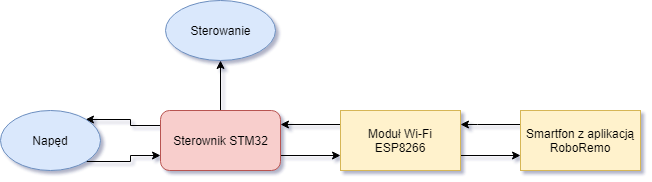
\includegraphics[width=0.8\textwidth]{figures/diagram.png}
	\caption{Architektura systemu}
	\label{fig:Architektura}
\end{figure}

%Obecne we wszystkich dokumentach
\section{Konfiguracja mikrokontrolera}

\begin{figure}[H]
	\centering
	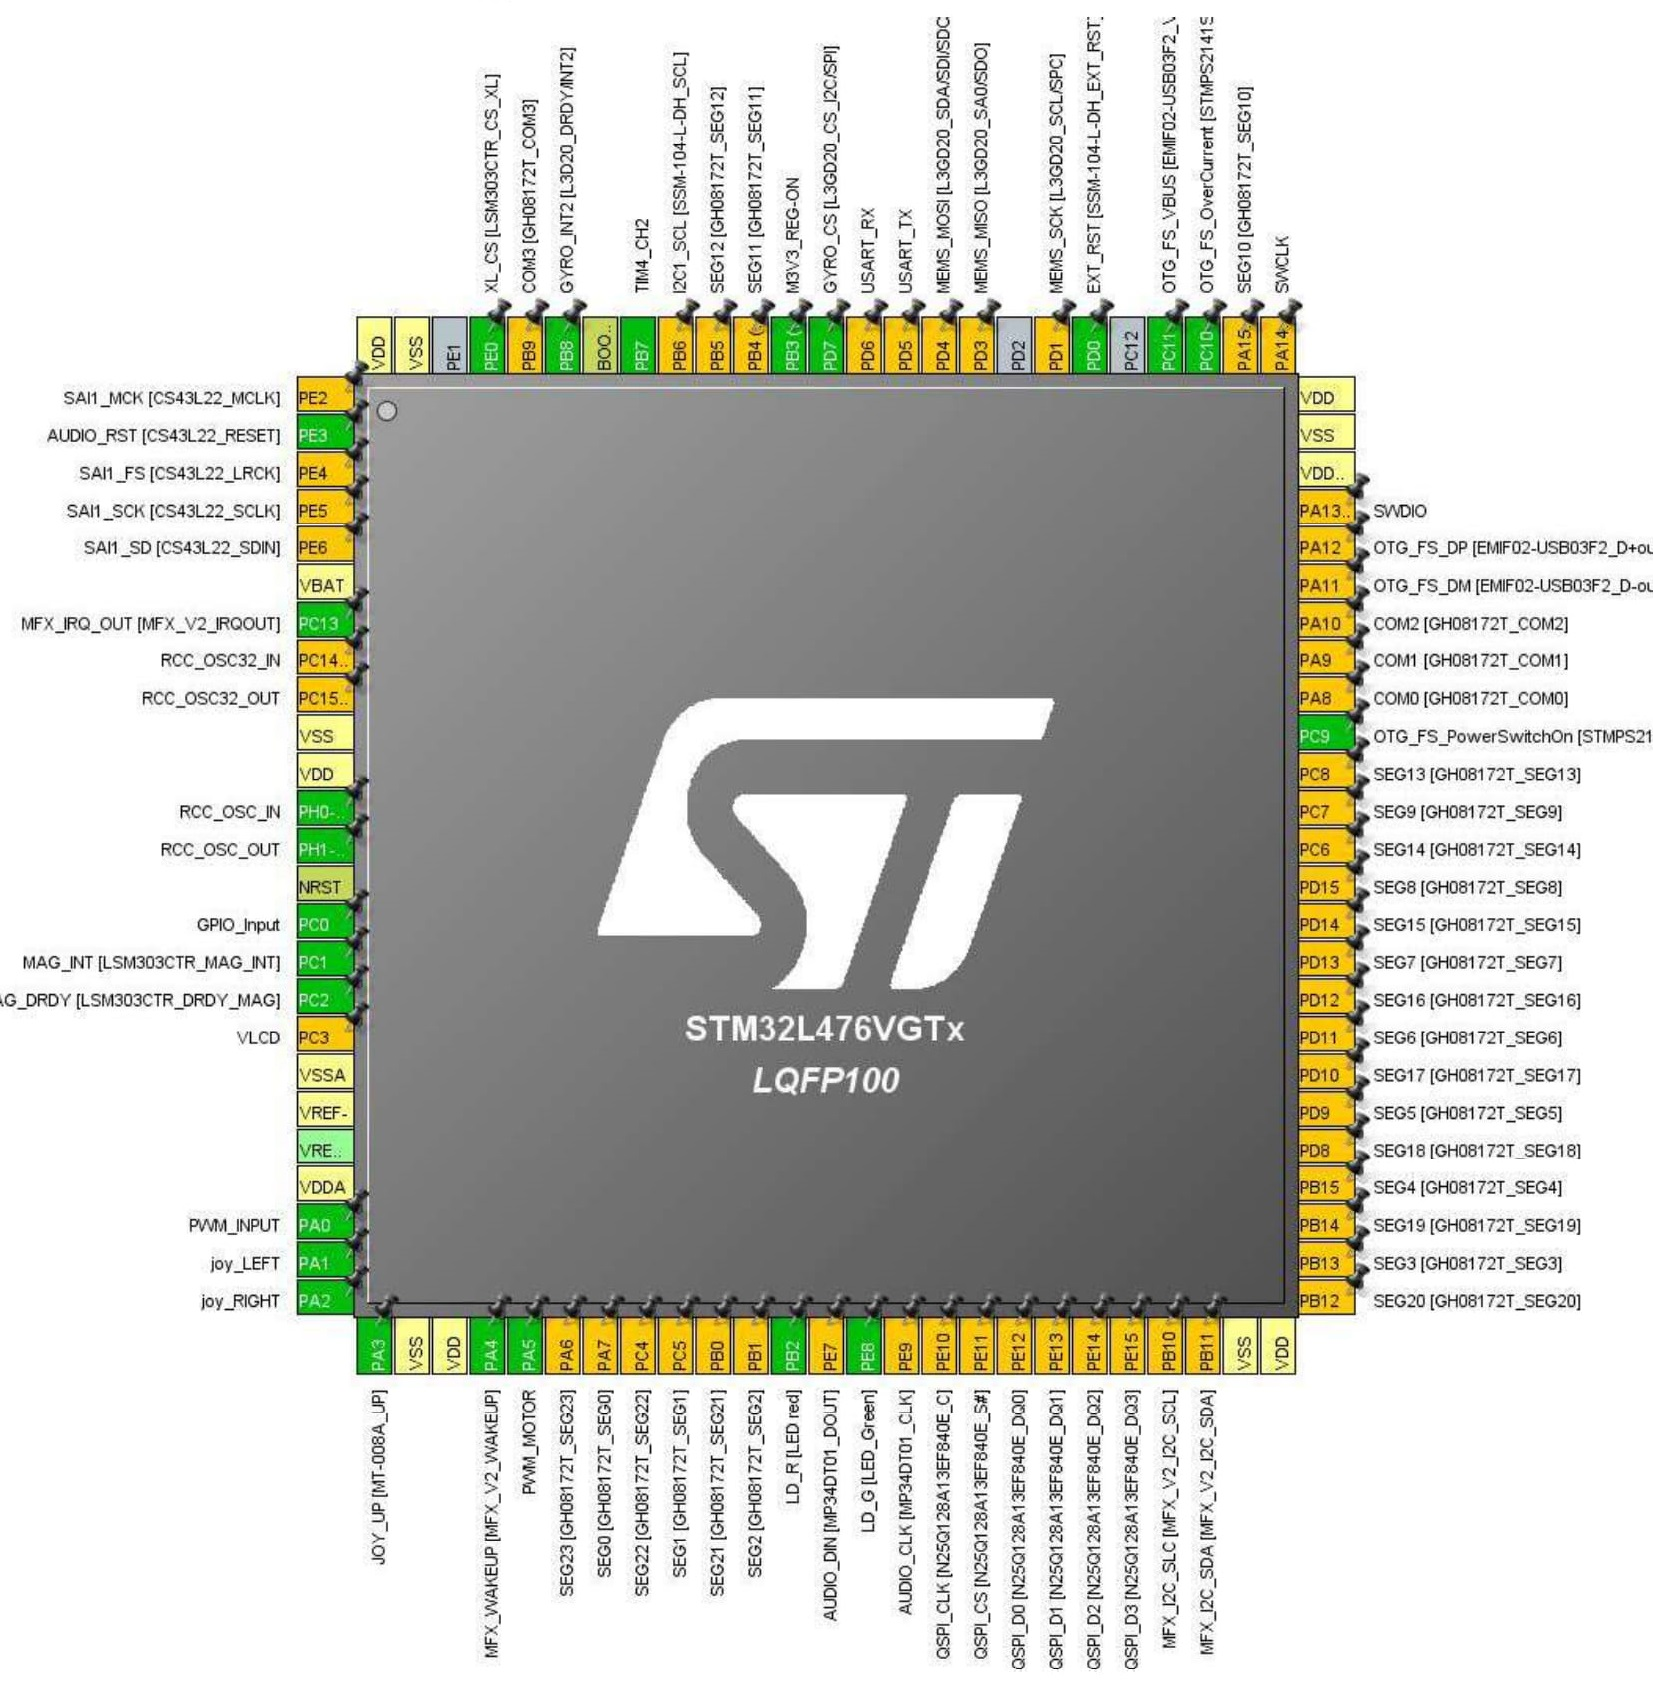
\includegraphics[width=1\textwidth]{figures/schemat-1.jpg}
	\caption{Konfiguracja wyjść mikrokontrolera w programie STM32CubeMX}
	\label{fig:KonfiguracjaMikrokontrolera}
\end{figure}

\newpage
\begin{figure}[H]
	\centering
	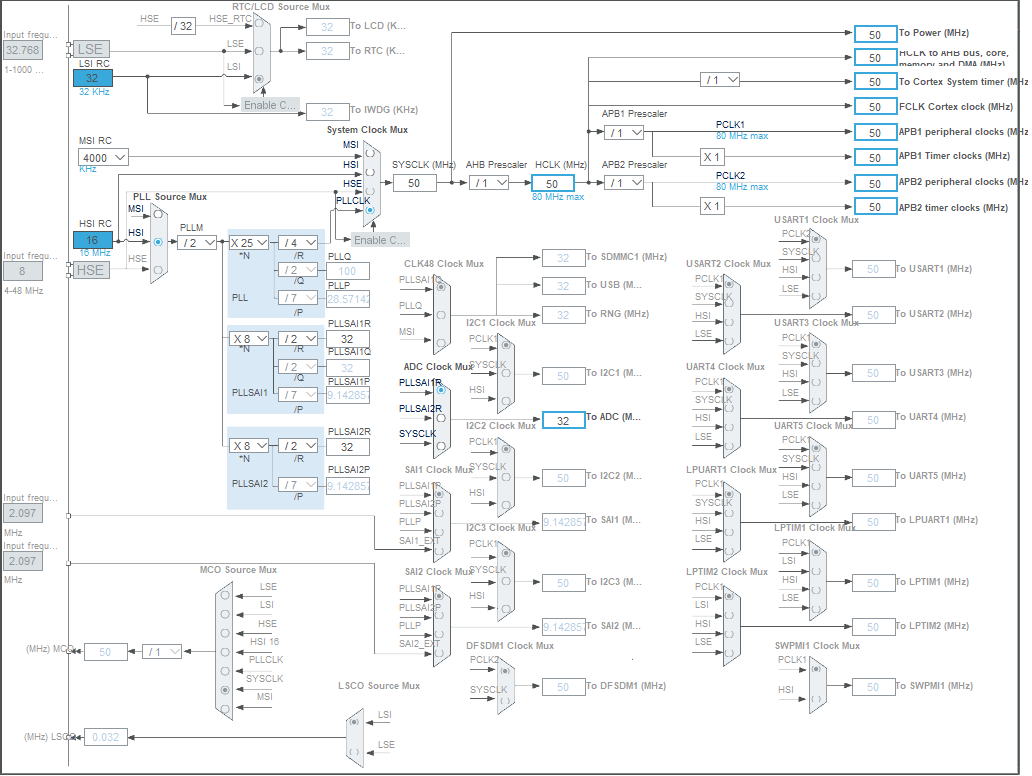
\includegraphics[width=0.9\textheight,angle=90]{figures/zegar.png}
	\caption{Konfiguracja zegarów mikrokontrolera}
	\label{fig:KonfiguracjaZegara}
\end{figure}

%Obecne we wszystkich dokumentach
\subsection{Konfiguracja pinów}

\begin{table}[H]
	\centering
	\begin{tabular}{|l|l|l|l|}
		\hline
		PIN & Tryb pracy & Funkcja/etykieta\\
		\hline
		PC14 & OSC32\_IN*	RCC\_OSC32\_IN	&\\
		PC15 & OSC32\_OUT*	RCC\_OSC32\_OUT	&\\
		PH0&  OSC\_IN*	RCC\_OSC\_IN	&\\
		PH1&  OSC\_OUT*&		RCC\_OSC\_OUT	\\
		PD5&	USART2\_TX&	USART\_TX\\
		PD6&	USART2\_RX&	USART\_RX\\
		%PE11&	TIM1\_CH2&	PWM\_SERVO\\
		PA0&	ADC1\_IN5&	PWM\_INPUT\\
		PA1&	GPIO\_Input&	JOY\_LEFT\\
		PA2&	GPIO\_Input&	JOY\_RIGHT\\
		PA3&	GPIO\_Input&	JOY\_UP\\
		PA4& GPIO\_Input& JOY\_DOWN\\
		PA5&	TIM2\_CH1&	PWM\_MOTOR\\
		PB7&    TIM4\_CH2&	PWM\_SERVO\\
		
		
		\hline
	\end{tabular}
	\caption{Konfiguracja pinów mikrokontrolera}
\end{table}

%Obecne we wszystkich dokumentach
\subsection{ADC 1}

\begin{table}[H]
	\centering
	\begin{tabular}{|l|c|} \hline
		\textbf{Parametr} & Wartość \\
		\hline
		\hline  \textbf{Resolution}&ADC 12-bit resolution  \\\hline
		\textbf{DMA Continuous Requests} & \textcolor{blue}{Enabled}\\\hline
		\textbf{Data Alignment} &  Right alignment\\
		\hline
		\textbf{Continuous Conversion Mode}& Disabled\\
		\hline
		\textbf{Channel}& Channel 5\\
		\hline
		\textbf{Sampling Time}& \textcolor{blue}{92.5 Cycles}\\
		\hline
	\end{tabular}
	\caption{Konfiguracja peryferium ADC}
	\label{tab:ADC}
\end{table}

\subsection{Timer 2}

\begin{table}[H]
	\centering
	\begin{tabular}{|l|c|} \hline
		\textbf{Parametr} & Wartość \\
		\hline
		\hline  \textbf{Clock Source}&Internal Clock  \\\hline
		\textbf{Channel1} & PWM Generation CH1\\\hline
		\textbf{Prescaler} & \textcolor{blue}{PWM\_PRESC}\\\hline
		\textbf{Counter Mode} &  Up\\
		\hline
		\textbf{Counter Period}& \textcolor{blue}{PWM\_PERIOD}\\\hline
		\textbf{Internal Clock Division}& No Division\\
		\hline
		\textbf{Mode}& PWM mode 1\\
		\hline
		\textbf{CH Polarity}& High\\
		\hline
	\end{tabular}
	\caption{Konfiguracja peryferium Timer 2}
	\label{tab:Timer2}
\end{table}

\subsection{Timer 4}

\begin{table}[H]
	\centering
	\begin{tabular}{|l|c|} \hline
		\textbf{Parametr} & Wartość \\
		\hline
		\hline  \textbf{Clock Source}&Internal Clock  \\\hline
		\textbf{Channel} & PWM Generation CH2\\\hline
		\textbf{Prescaler} & \textcolor{blue}{999}\\\hline
		\textbf{Counter Mode} &  Up\\
		\hline
		\textbf{Counter Period}& \textcolor{blue}{999}\\\hline
		\textbf{Internal Clock Division}& No Division\\
		\hline
		\textbf{Mode}& PWM mode 1\\
		\hline
		\textbf{CH Polarity}& High\\
		\hline
	\end{tabular}
	\caption{Konfiguracja peryferium Timer 4}
	\label{tab:Timer4}
\end{table}

\subsection{Timer 6}

\begin{table}[H]
	\centering
	\begin{tabular}{|l|c|} \hline
		\textbf{Parametr} & Wartość \\
		\hline
		\hline
		\textbf{Prescaler} & \textcolor{blue}{TIM6\_PRESC}\\\hline
		\textbf{Counter Mode} &  Up\\
		\hline
		\textbf{Counter Period}& \textcolor{blue}{TIM6\_PERIOD}\\\hline
		\textbf{Trigger Event Selection}& \textcolor{blue}{Update Event}\\
		\hline
	\end{tabular}
	\caption{Konfiguracja peryferium Timer 6}
	\label{tab:Timer6}
\end{table}
%Obecne w dokumencie do etapu II oraz III
%\section{Urządzenia zewnętrzne}
%\textcolor{red}{Rozdział ten powinien zawierać opis i konfigurację %wykorzystanych ukladów
%	zewnętrznych, jak np. akcelerometr.}


%Obecne w dokumencie do etapu II oraz III
\section{Projekt elektroniki}
	\subsection{Schemat elektryczny}
	\begin{figure}[H]
		\centering
		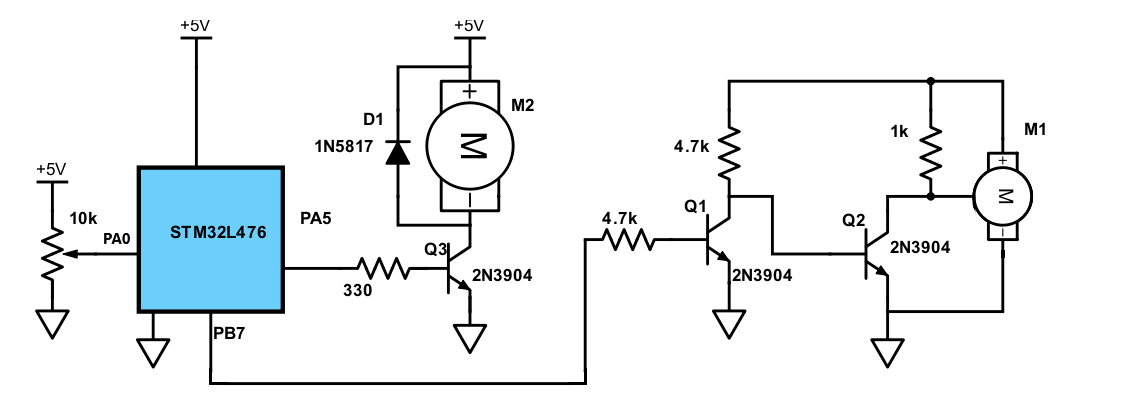
\includegraphics[width=1\textwidth]{figures/schemeit-project.png}
		\caption{Schemat elektryczny}
		\label{fig:Schemat elektryczny}
	\end{figure}
	
\subsection{Regulacja prędkości napędu}
Za pomocą potencjometru regulujemy wypełnienie sygnału PWM. Sygnał ten jest wzmacniany za pomocą tranzystora NPN i przekazywany do silnika DC.

\begin{figure}[H]
	\centering
	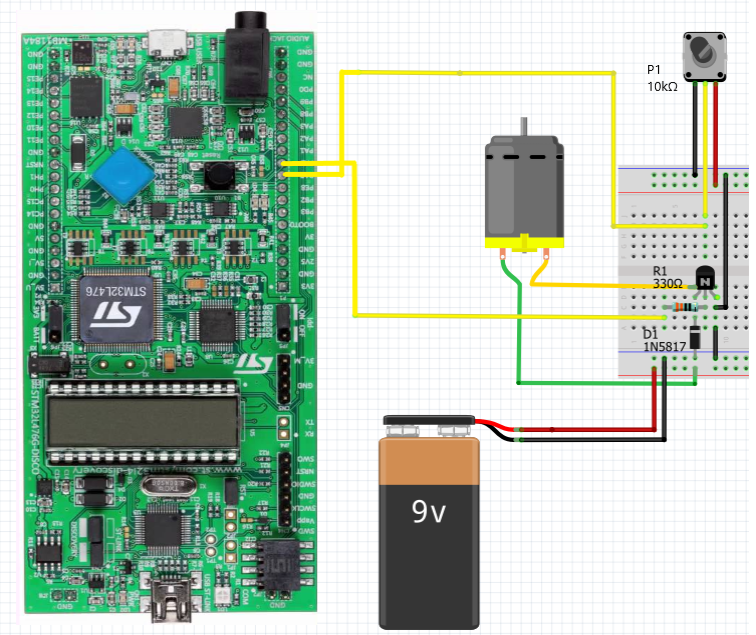
\includegraphics[width=0.8\textwidth]{figures/pwm.png}
	\caption{Schemat poglądowy regulacji prędkości obrotowej silnika}
	\label{fig:KonfiguracjaPWM}
\end{figure}

%Obecne w dokumencie do etapu II oraz III
\section{Konstrukcja mechaniczna}

	\begin{figure}[H]
		\centering
		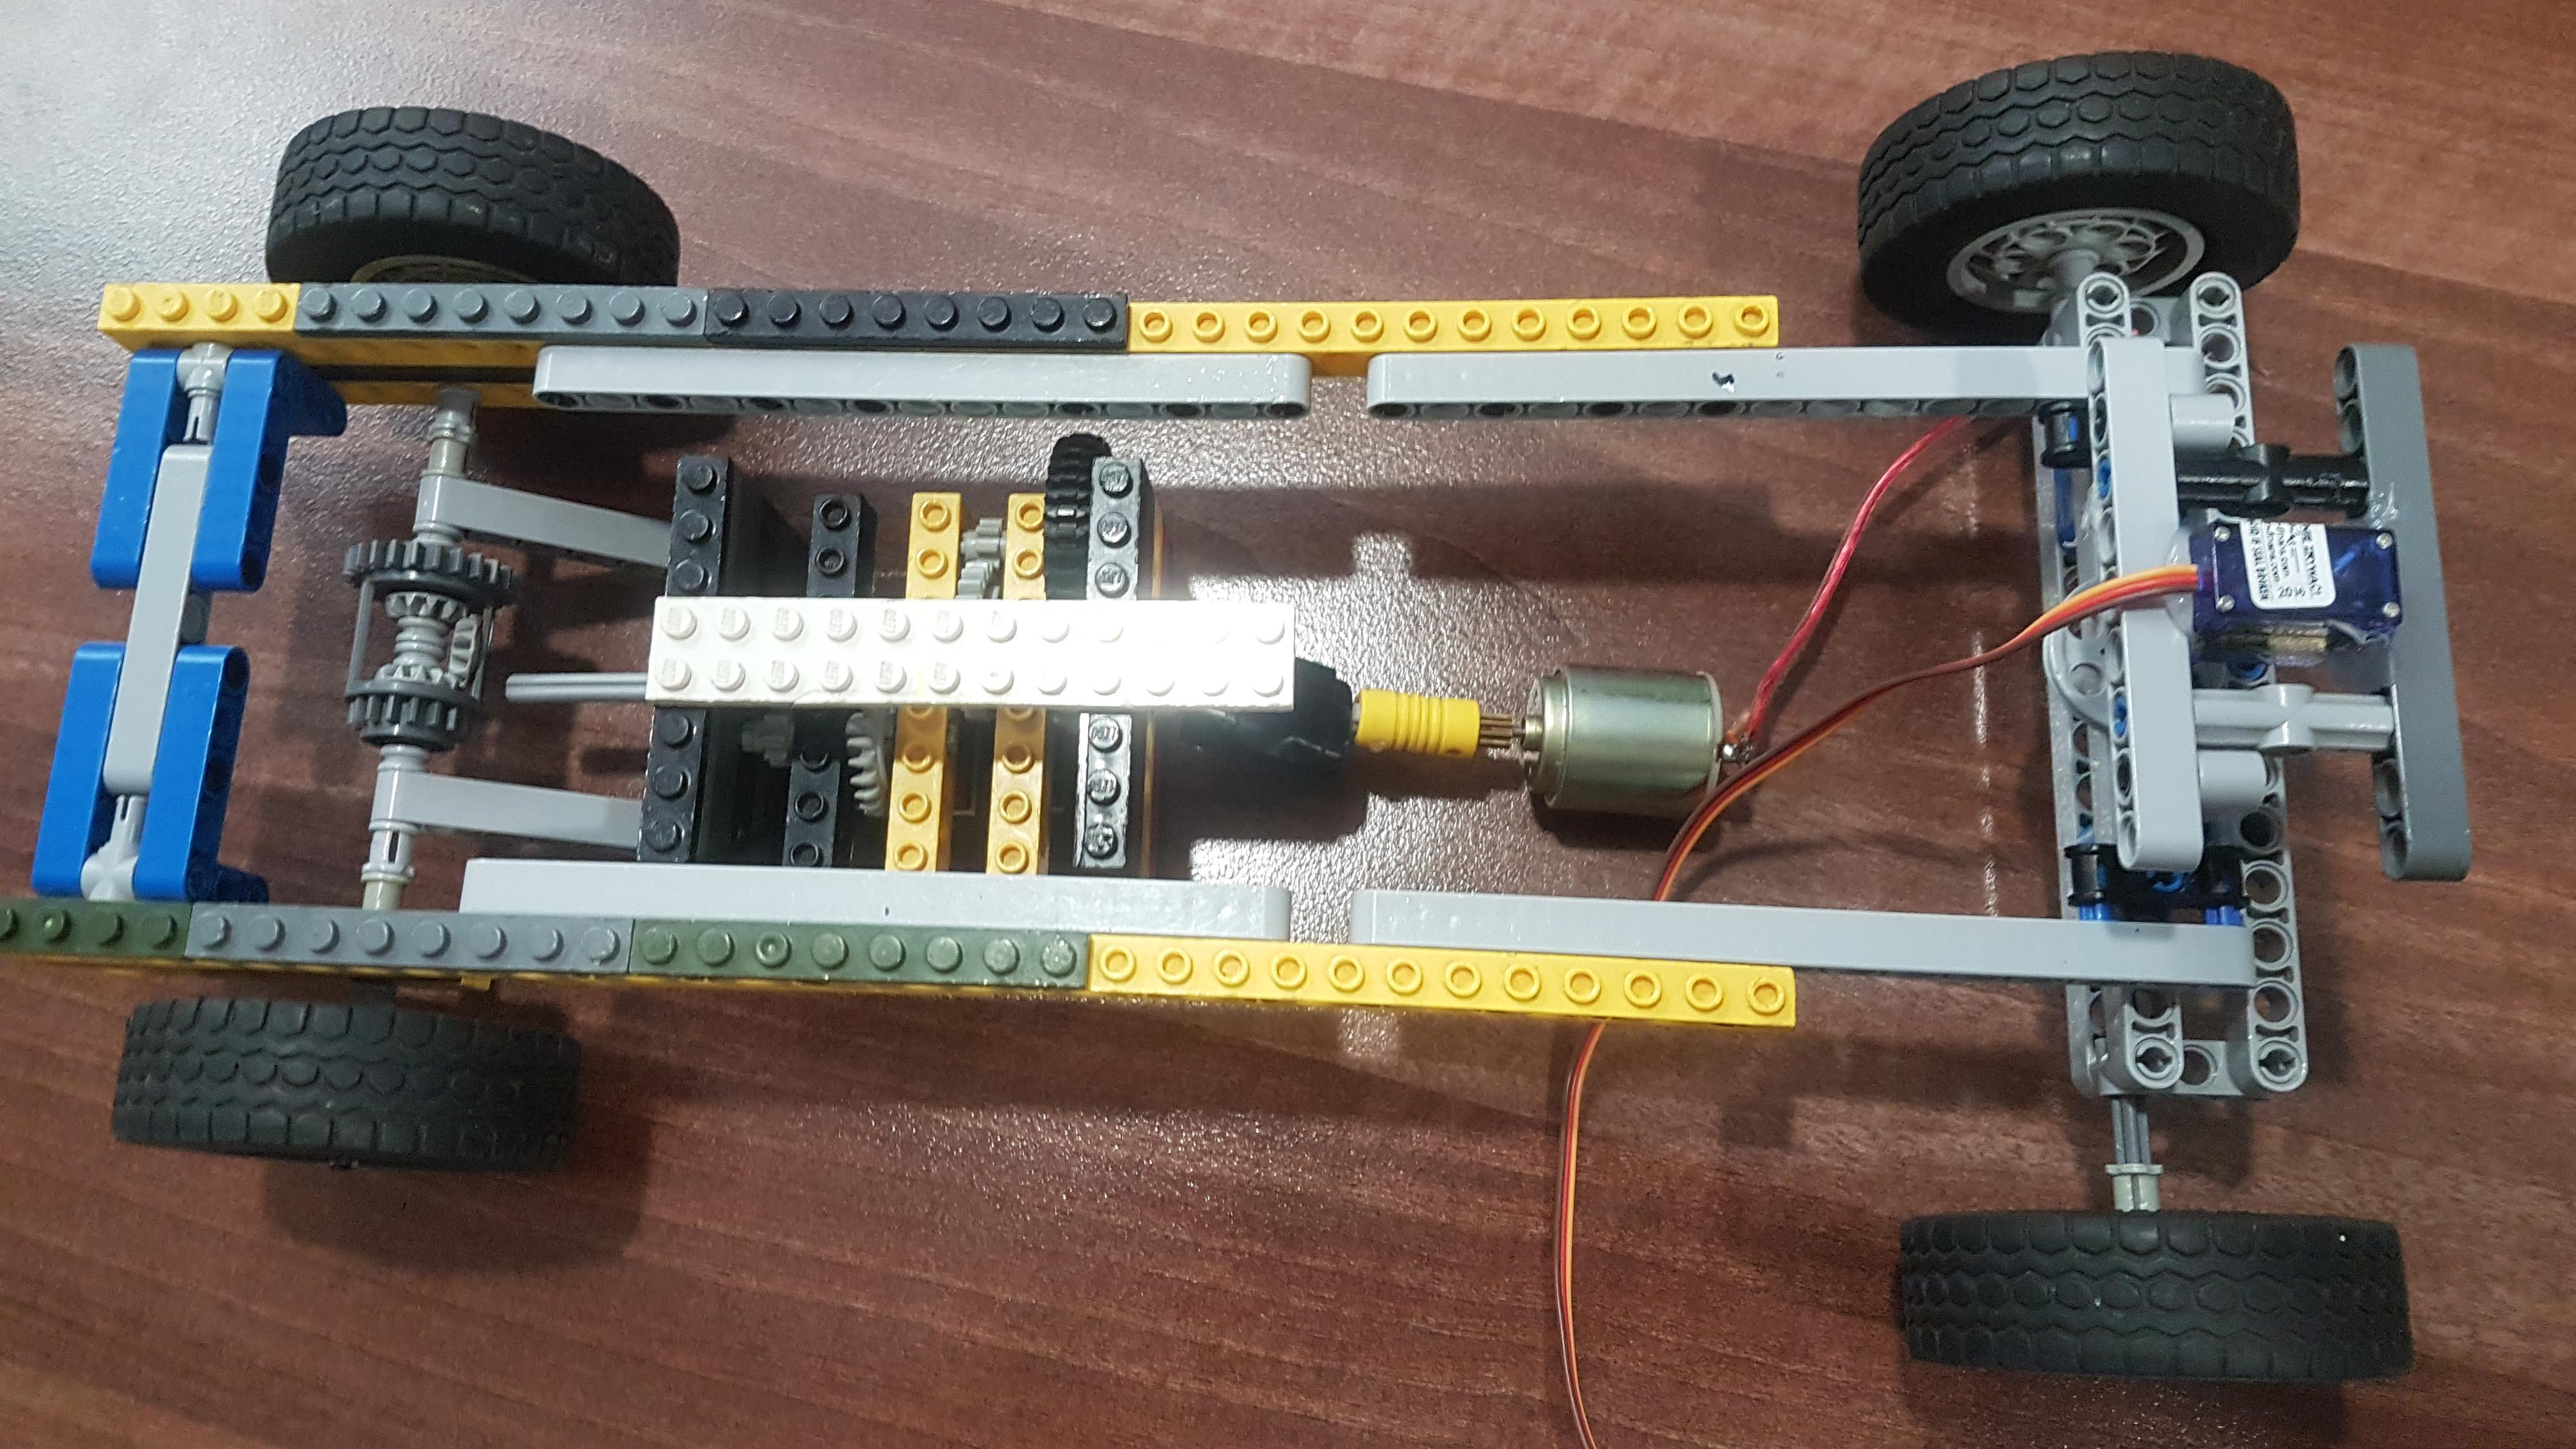
\includegraphics[width=1\textwidth]{figures/20190410_135905.jpg}
		\caption{Zdjęcie części mechanicznej nr 1}
		\label{fig:Zdjęcie części mechanicznej nr 1}
	\end{figure}
	
		\begin{figure}[H]
		\centering
		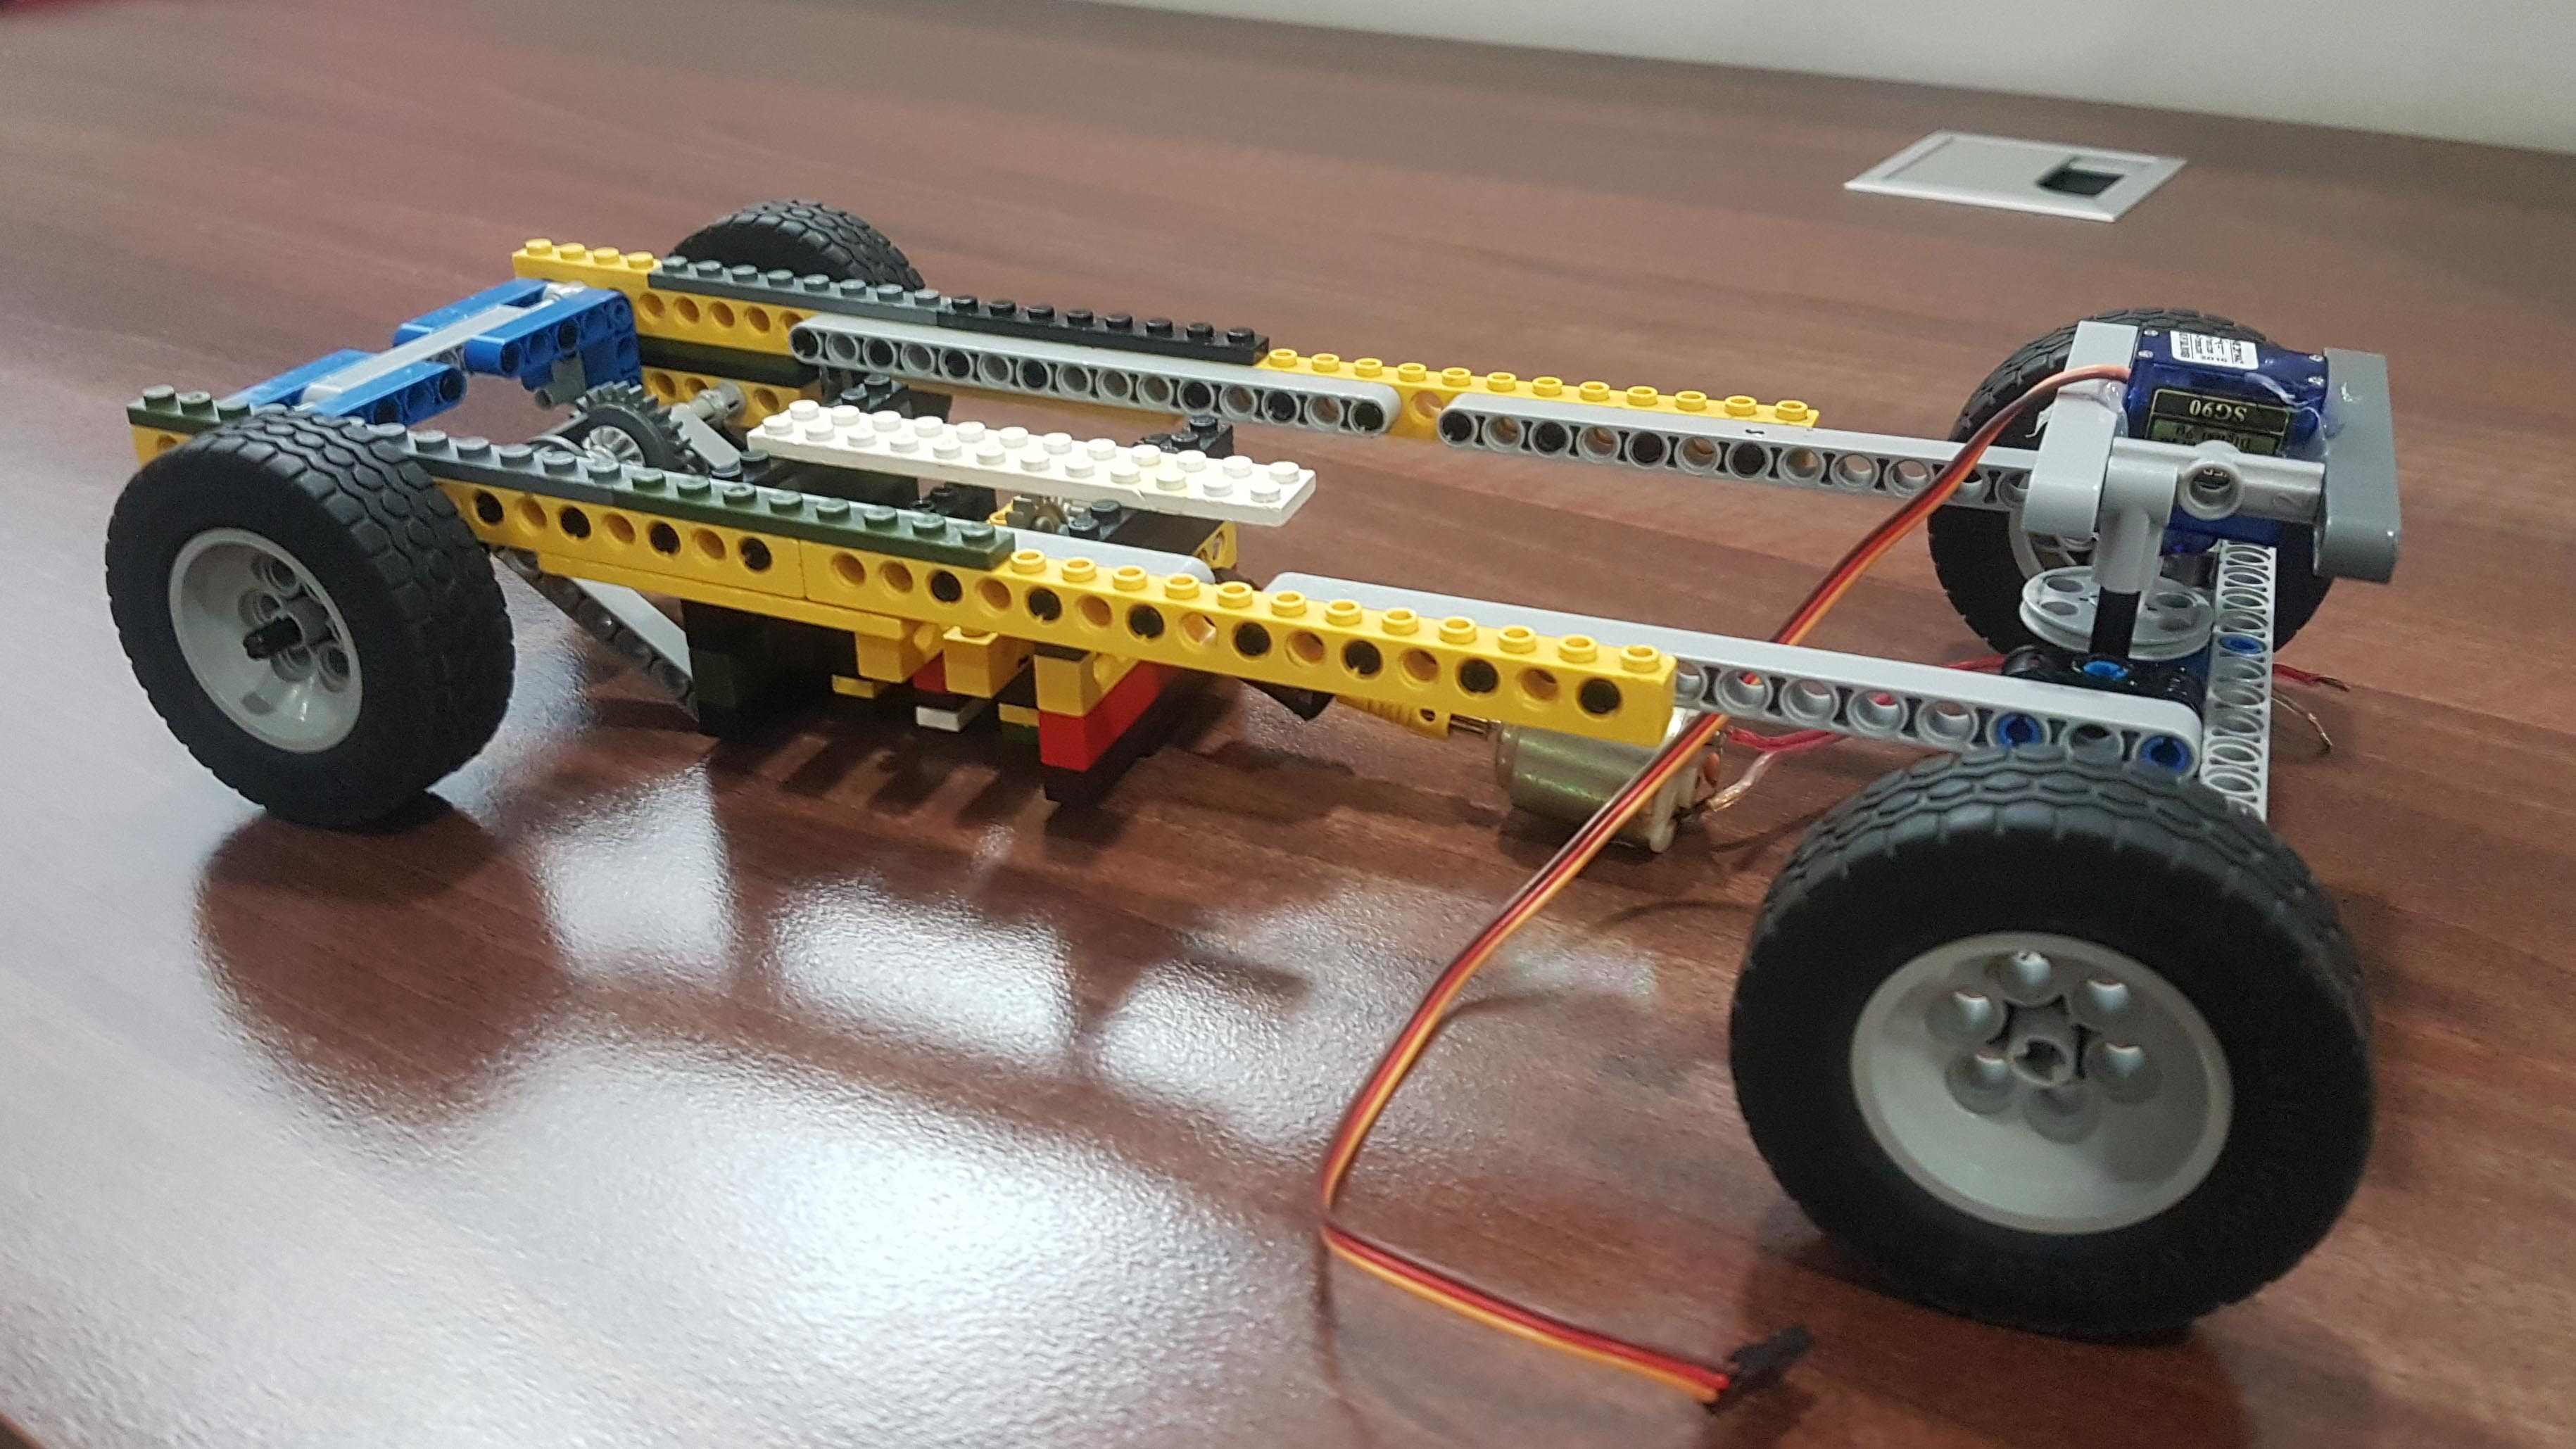
\includegraphics[width=1\textwidth]{figures/20190410_135853.jpg}
		\caption{Zdjęcie części mechanicznej nr 2}
		\label{fig:Zdjęcie części mechanicznej nr 2}
	\end{figure}

%Obecne w dokumencie do etapu II oraz III
\section{Opis działania programu}

\subsection{Schemat działania programu}
	\begin{figure}[H]
		\centering
		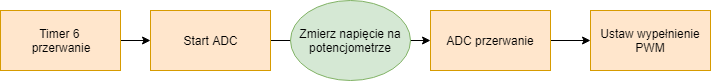
\includegraphics[width=0.8\textwidth]{figures/diagramPWM.png}
		\caption{Schemat działania programu}
		\label{fig:diagramPWM}
	\end{figure}

\subsection{Funkcja obsługująca przerwanie timera 6}
	\begin{lstlisting}[tabsize=2]
	void HAL_TIM_PeriodElapsedCallback(TIM_HandleTypeDef *htim)
	{
		if(htim->Instance == TIM6)
			HAL_ADC_Start_DMA(&hadc1, (uint32_t *)&adc_value, 1);
	}
	\end{lstlisting}

\subsection{Funkcja obsługująca przerwanie ADC}
\begin{lstlisting}[tabsize=2]
void HAL_ADC_ConvCpltCallback(ADC_HandleTypeDef* hadc)
{
	//pid_output = pid_calc(&pid, adc_value, set_value);
	__HAL_TIM_SET_COMPARE(&htim2 , TIM_CHANNEL_1, adc_value);
}
\end{lstlisting}

%Obecne w dokumencie do etapu II oraz III (jeśli coś zostało niezrealizowane)
\section{Zadania niezrealizowane}
Nie zostało zrealizowane przekazanie napędu z silnika i serwomechanizmu na mechanizm napędowy oraz na ten służący do skręcania. W pierwszym przypadku jest to spowodowane brakiem czasu, wynikający ze zbyt długim poszukiwaniem rozwiązania na problem przeniesienia napędu z silnika do przekładni, natomiast w drugim tym, że wał serwomechanizmu ma stępione zębatki co uniemożliwia przekazanie jakiejkolwiek siły na dalszy podzespół.

%Obecne we wszystkich dokumentach
\section{Podsumowanie}

Udało się zrealizować większość zadań. Nastąpiły drobne zmiany koncepcyjne jak użycie potencjometru do regulacji prędkości obrotowej napędu. To będzie wymagać mniejszej ingerencji gdy będziemy projektować regulator PID.

\newpage
\addcontentsline{toc}{section}{Bibilografia}
\bibliography{bibliografia}
\bibliographystyle{plabbrv}


\end{document}







































